\chapter{Softwarearchitektur des Java Medical Imaging Toolkit} \label{architecture}
\addthumb{Softwarearchitektur des Java Medical Imaging Toolkit}{\huge{\textbf{\thechapter.}}}{white}{haw_rot} 

\section{Die Eclipse Rich Client Platform}

Die Grundlage für eine modulare Entwicklung der Software liefert die Eclipse Rich Client\footnote{Es lässt sich zwischen Rich Clients und Thin Clients unterscheiden. Rich Clients stellen sowohl die Präsentationsschicht als auch die logische Schicht auf dem Client zur Verfügung. Die Applikationsfunktionalität der Thin Clients wird komplett von einem Server bereitgestellt. Die Bedienung erfolgt meist über den Browser.} Platform (RCP). Eclipse, basierend auf der Programmiersprache Java, wird seit 2001 von einer OpenSource-Gemeinde entwickelt\cite{vogel:eclipseoverview}. Während es anfangs rein für die Java-Applikationsentwicklung entworfen wurde, ist es heute eine allgemeine erweiterbare Entwicklungsumgebung. So lässt sich zum einen das Grundprogramm mit Hilfe sogenannter Plug-ins erweitern und zum anderen eigenständige Applikationen erstellen (RCP), die auf dem Eclipse-Framework aufbauen. Das \glqq Aptana Studio\grqq\footnote{http://www.aptana.com/} ist beispielsweise ein Plug-in, das der Grundentwicklungsumgebung mehrere Funktionalitäten im Bereich der Webentwicklung (Kommunikation zum Server, Syntaxhighlighting von HTML und CSS) hinzufügt. \glqq RSS Owl\grqq\footnote{http://www.rssowl.org/}, ein Programm zur Verwaltung von Newsfeeds, ist ein Beispiel für eine eigenständige Rich Client Applikation auf Basis von Eclipse.\\
Eine Kernkomponente des Eclipse-Frameworks ist \textit{Equinox}, eine Implementierung der OSGi-Spezifikation. OSGi bietet die Möglichkeit, modulare Java-Applikationen zu entwickeln und Softwarepakete (nach der Spezifikation \glqq Bundles\grqq\, unter Eclipse \glqq Plug-ins\grqq\ genannt) während der Laufzeit hinzuzufügen, zu entfernen, zu starten oder zu stoppen \cite{vogel:e4overview}. Das Java Medical Imaging Toolkit ist eine Implementierung eines Bundles, beziehungsweise Plug-ins.\\
Abbildung \ref{eclipsee4arch} zeigt die Architektur der Eclipse Rich Client Platform.

\begin{figure}[htbp]
  \vspace{0.5cm}
  \centering
  \fbox{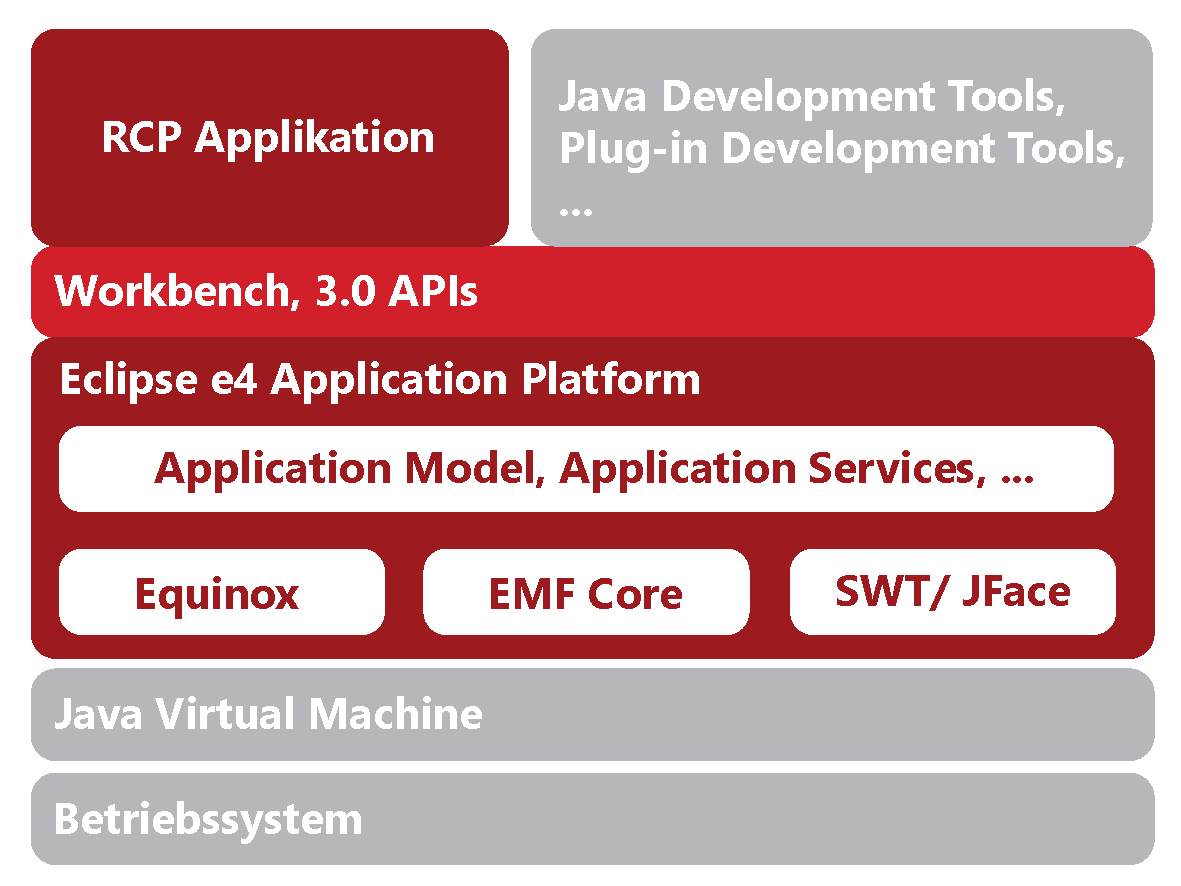
\includegraphics[angle=0,width=10cm]{./img/e4arch.pdf}}
  \caption{Architektur der Eclipse e4 Plattform zur Entwicklung von Rich Client Applikationen \cite{e4:screen}}
  \label{eclipsee4arch}
  \vspace{0.5cm}
\end{figure}

Die untere Ebene bildet das Betriebssystem. Eclipse kann grundsätzlich plattformunabängig unter Windows, verschiedener Linux Distributionen oder Mac OS eingesetzt werden. Einzige Voraussetzung ist eine installierte Java Virtual Machine. Aufbauend auf Java steht der Eclipse-Kern, bestehend aus dem OSGi-Framework Equinox, dem Eclipse Modeling Framework EMF\footnote{Das EMF dient beispielsweise zur Entwicklung eines Datenmodells, wird allerdings für weitere Ausführungen nicht explizit benötigt.} und dem Standard Widget Toolkit SWT und dient als Standardwerkzeug zur Erstellung der Benutzeroberfläche. Das SWT ist eine OpenSource Implementierung verschiedenster grafischer Bedienelemente wie Schaltflächen, Textfelder, Tabellen und vieles mehr. Der Unterschied zu den in Java integrierten grafischen Oberflächen besteht darin, dass das Standard Widget Toolkit auf die Ressourcen des Betriebssystems zugreift und sich in der Darstellung den Betriebssystemstandards anpasst\cite{eclipse:swt}.In Eclipse Rich Clients Applikationen ersetzt das SWT das Java-eigene AWT und Swing). Aufbauend auf den Grundkomponenten liegt das \textit{Application Model}, das die Struktur der Applikation(Menüs, Fenster, etc.) beschreibt \cite[Kapitel 7]{vogel:e4overview}.\\
Workbench und Eclipse 3.0 APIs bieten noch die Möglichkeit Anwendungen abwärtskompatibel zu entwickeln. Die gesamte Plattform bildet die Basis für das Java Medical Imaging Toolkit. Durch das Application Model kann modular entwickelt und die Programmstruktur in zukünftigen Versionen erweitert werden.

\section{Das Eclipse Application Model}

Damit eine Anwendung strukturiert werden kann stellt das Application Model steuernde und visuelle Elemente zur Verfügung. Das bedeutet, dass das Application Model den Aufbau der Anwendung, wie zum Beispiel die Andordnung der einzelnen Elemente, regelt und die Implementierung an anderer Stelle stattfindet.

\begin{itemize}

\item \textbf{Strukturen zur visuellen Beschreibung der Applikation}\\
	Das Aussehen wird mit Hilfe von Windows, Parts, PartStacks und anderen Elementen des Application Models beschrieben. Die Elemente enthalten noch keine Logik sondern definieren nur die Struktur der Anwendung.


\item \textbf{Strukturen zur Steuerung des Verhaltens}\\
	 Zu den Komponenten die das Verhalten der Applikation beeinflussen zählen zum Beispiel Tastatur-Shortcuts, Commands und Handler. Letztere dienen zur Verarbeitung von Benutzereingaben.

\end{itemize}

\subsection{Visuelle Komponenten}

\subsubsection{Window}
Windows sind einfache Repräsentationen eines Fensters der Benutzeroberfläche\cite[org.eclipse.e4.ui.model.application.ui.basic]{eclipse:help}. Sie bilden das Grundgerüst der Applikation und beinhalten Perspectives, PartStacks und andere Elemente. Ein einfaches Fenster ist in Abbildung \ref{rcp_window} zu sehen.

\subsubsection{Menüs}
Ein Menü ist der Container für verschiedene Menü-Elemente und dient dazu, Benutzereingaben entgegenzunehmen. Einem Element können Commands hinterlegt werden, damit die Eingaben weiter verarbeitet werden können. Ein Menüpunkt kann selbst ein Menü beinhalten.

\subsubsection{Perspective}
Perspectives beinhalten eine Menge von Elementen der Benutzeroberfläche wie PartStacks und Parts. Perspectives können unabhängig vom Rest der Oberfläche gewechselt werden\cite[org.eclipse.e4.ui.model.application.ui.advanced]{eclipse:help}. So können Perspectives beispielsweise die Anordnung der Parts definieren  oder neue Parts anzeigen, die in einer anderen Perspective nicht enthalten sein sollen. Unter Eclipse hat zum Beispiel das Debug-Modul eine eigene Perspective und es kann dynamisch zwischen Debug- und Entwicklungsperspektive gewechselt werden.

\subsubsection{PartSashContainer}
Wie der Name bereits andeutet, ist ein PartSashContainer ein Container für PartStacks und Parts. Die enthaltenen Elemente werden komplett angezeigt. In Abbildung \ref{rcp_partsash} ist eine solche Kombination zu sehen. Die obere Hälfte stellt einen PartStack mit den beiden Parts \textit{TestPart A} und \textit{TestPart B} dar. Der Untere Teil ist ein Stack-unabhängiger Part.

\subsubsection{PartStack}
Auch der PartStack dient als Behälter für einzelne Parts. Der Unterschied zum PartSashContainer liegt darin, dass bei PartStacks nur der aktuell ausgewählte Part angezeigt wird. Die Darstellung des Stacks ist mit üblichen Tabs zu vergleichen, wie Abbildung \ref{rcp_partStack} zeigt. Der Stack enthält die beiden Parts \textit{TestPart A} und \textit{TestPart B}.

\subsubsection{Part}
Ein Part ist die kleinste Einheit des Application Models und ist Kern der Benutzeroberfläche\cite[org.eclipse.e4.ui.model.application.ui.basic]{eclipse:help}. Innerhalb der Parts werden alle weiteren Bedienelemente angezeigt. Jede Abbildung von \ref{rcp_part} - \ref{rcp_partsash} enthält eine oder mehrere Parts. Betrachtet man das Application Model als Baumstruktur, symbolisieren Parts die Blattknoten. Parts können direkt einem Window unterstellt oder tief verschachtelt zwischen Perspectives und Stacks benutzt werden.


\subsection{Steuernde Komponenten}
\subsubsection{Commands}
Commands bilden die abstrakte Schicht zwischen Benutzereingabe und Verarbeitung. Commands besitzen keine eigene Implementierung. Das ermöglicht dem Entwickler das Verhalten indiviuell zu gestalten. So könnte ein Einfügen-Befehl im Editor ein anderes Verhalten auslösen als im Explorer-Part\cite[org.eclipse.ui.commands]{eclipse:help}.

\subsubsection{Handler}
Handler sind die konkreten Implementierungen der Commands und sind für die Verarbeitung der Benutzereingaben verantwortlich.

\begin{figure*}
%\subfigure[Keypoints]{\includegraphics[width=0.49\textwidth]{./img/basmati_keypoints.png}}\hfill
%\centering

\subfigure[Window]{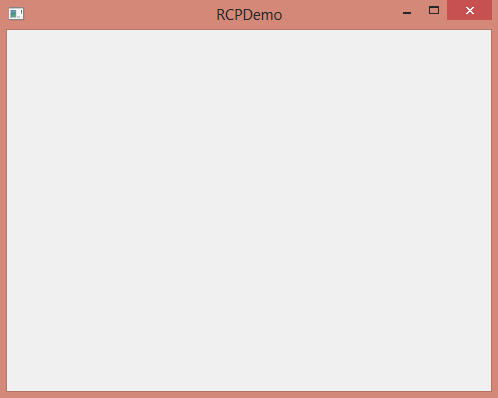
\includegraphics[width=0.40\textwidth]{./img/rcp_window.png} \label{rcp_window}}\hfill
\subfigure[Part]{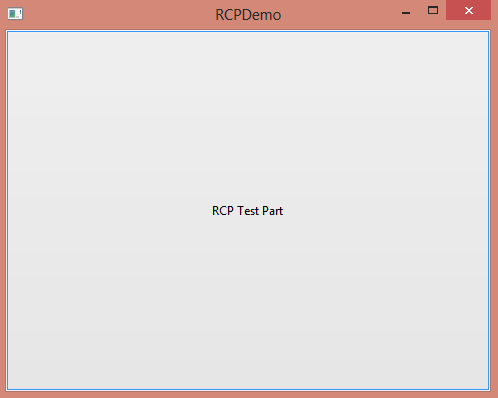
\includegraphics[width=0.40\textwidth]{./img/rcp_part.png} \label{rcp_part}}\\
\subfigure[PartStack]{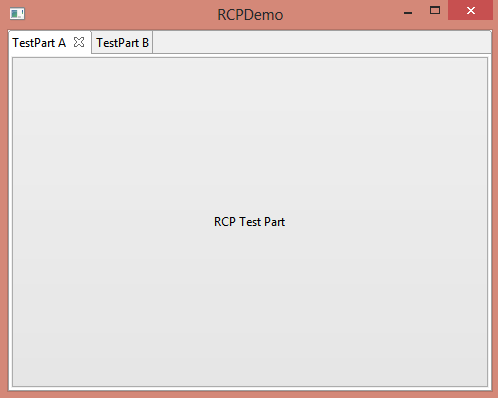
\includegraphics[width=0.40\textwidth]{./img/rcp_partStack.png} \label{rcp_partStack}}\hfill
\subfigure[PartSashContainer]{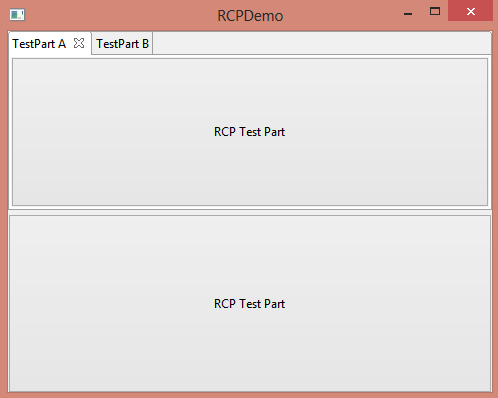
\includegraphics[width=0.40\textwidth]{./img/rcp_partsash.png} \label{rcp_partsash}}

\caption{Verschiedene Elemente des Application Models}
\label{rcp_example}
\end{figure*}

\section{Die Benutzeroberfläche von jMediKit} \label{jmedikit_structure}

Die Oberfläche des Java Medical Imaging Toolkit besteht aus sechs zentralen Elementen, um den Anforderungen zur Darstellung und Bedienung zu entsprechen.
\begin{enumerate}
\item \textbf{Hauptmenü} \\
	  Das Hauptmenü stellt globale und bildspezifische Operationen zur Verfügung. So werden unter dem Menüpunkt \textit{Erweiterungen} die importierten Plug-ins aufgelistet.
\item \textbf{Werkzeugleiste} \\
	  Dieser Teil der Benutzeroberfläche stellt hauptsächlich Möglichkeiten zur Manipulation der Bilddaten zur Verfügung. Das Kapitel \glqq \ref{implementation}. \nameref{implementation}\grqq\ geht genau auf die verfügbaren Werkzeuge ein.
\item \textbf{DicomBrowser} \\
	  Dieser Part erlaubt die Navigation durch die vom Programm geladenen DICOM-Objekte. Die Anordnung entspricht der Darstellung des ER-Modells aus Kapitel \glqq \ref{grundlagen}. \nameref{grundlagen}\grqq\
\item \textbf{ImageView} \\
	 ImageView übernimmt die Anzeige der Pixeldaten der DICOM-Objekte.
\item \textbf{Console} \\
	Die Konsole dient der Fehlerausgabe bei der Plug-in-Entwicklung.
\item \textbf{DicomTagView} \\
	Im DicomTagView werden die Tags eines ausgewählten DICOM-Objekts dargestellt.
\end{enumerate}

\begin{figure}[htbp]
  \vspace{0.5cm}
  \centering
  \fbox{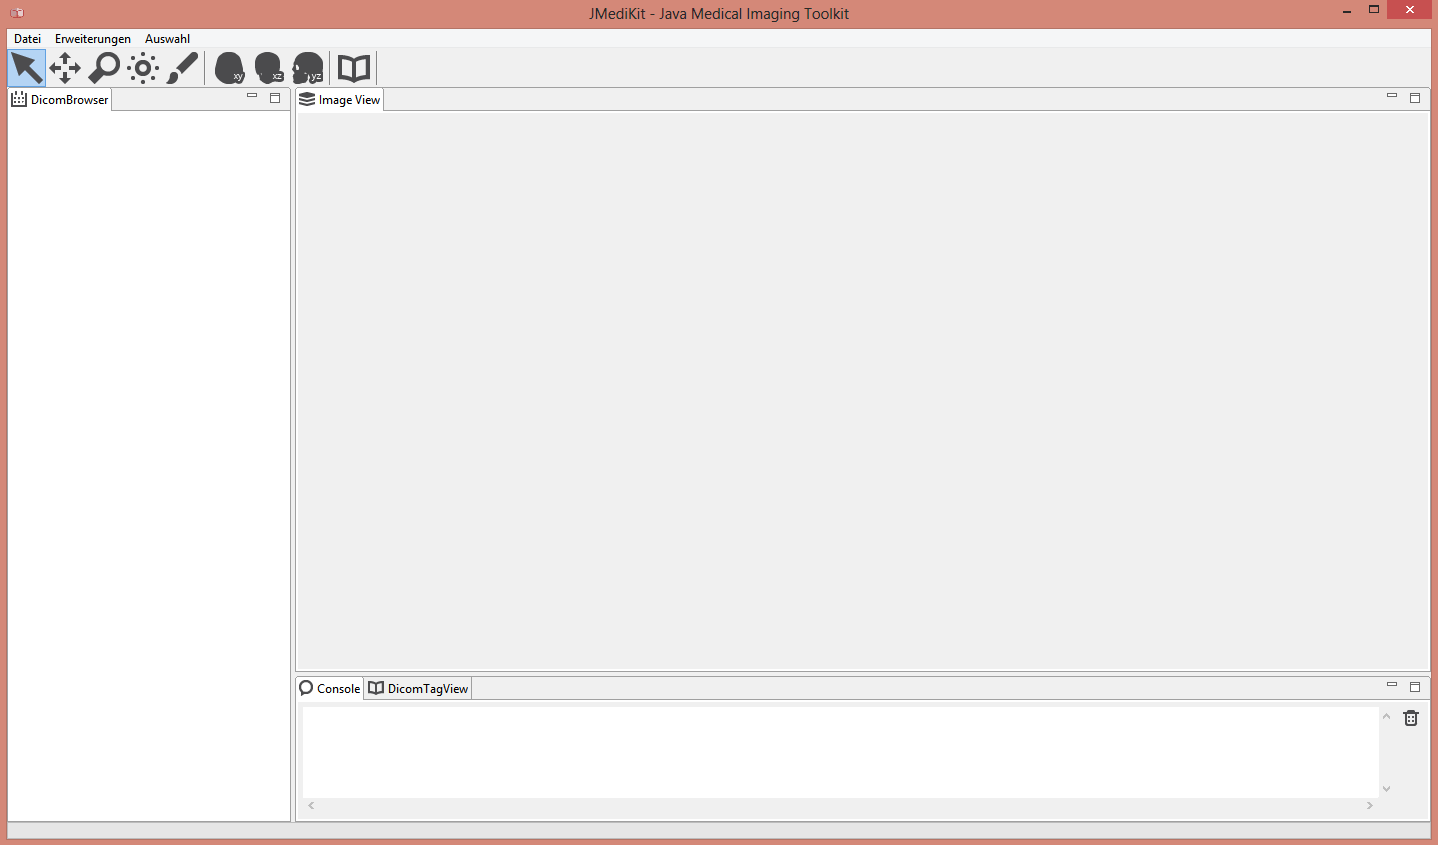
\includegraphics[angle=0,width=12cm]{./img/jmedikit_ui.png}}
  \caption{Die Benutzeroberfläche von jMediKit}
  %\floatfoot{https://wiki.eclipse.org/Eclipse4}
  \label{jmedikitui}
  \vspace{0.5cm}
\end{figure}

Die hierarchische Struktur der Anwendung wird in Abbildung \ref{hierarchy} dargestellt. Die sechs Blattknoten repräsentieren den nach außen für den Benutzer sichtbaren Teil der Anwendung. 


\section{Erweiterbarkeit der Grundstruktur} \label{hierarchyextending}
Die flexible Struktur des Eclipse Application Models und der Rich Client Platform erlauben komfortable Erweiterungen. So können einzelne Parts den schon bestehenden Elementen zugeordnet, oder neue Perspectives eingefügt werden, die eine neue Benutzeroberfläche abbilden könnten. Beispielsweise kann ein neuer Part den FileStack(Abbildung \ref{hierarchy}) damit erweitern, dass DICOM-Objekte von einem PACS geladen werden. Das Kapitel \glqq \ref{extending}. \nameref{extending}\grqq\ zeigt eine Möglichkeit, jMediKit einen neuen Part hinzuzufügen.\\
Durch das Hinzufügen von Elementen des Application Models ist es möglich, in die Struktur und vor allem die Benutzeroberfläche einzugreifen. Das bedeutet auch, dass Parts oder andere Strukturen nur in der Lage sind neue Funktionen einzubauen. Es fehlt die Möglichkeit bereits existierende Elemente wie das Hauptmenü (MainMenu) oder die Werkzeugleiste (Toolbar) zu erweitern.
%Damit ist der Teil erfüllt, dass die zu entwickelnde Anwendung für Erweiterungen offen steht. Modulare Werkzeuge %komplettieren die Anforderung der Erweiterbarkeit für Entwickler.

\tikzstyle{every node}=[draw=black,thick,anchor=south, align=center]
%\tikzstyle{selected}=[draw=red,fill=red!30]
\tikzstyle{optional}=[dashed,fill=gray!50]
\begin{figure}[htbp]
\centering
\caption{jMediKit und die hierarchische Anordnung der Elemente des Application Models}
\label{hierarchy}
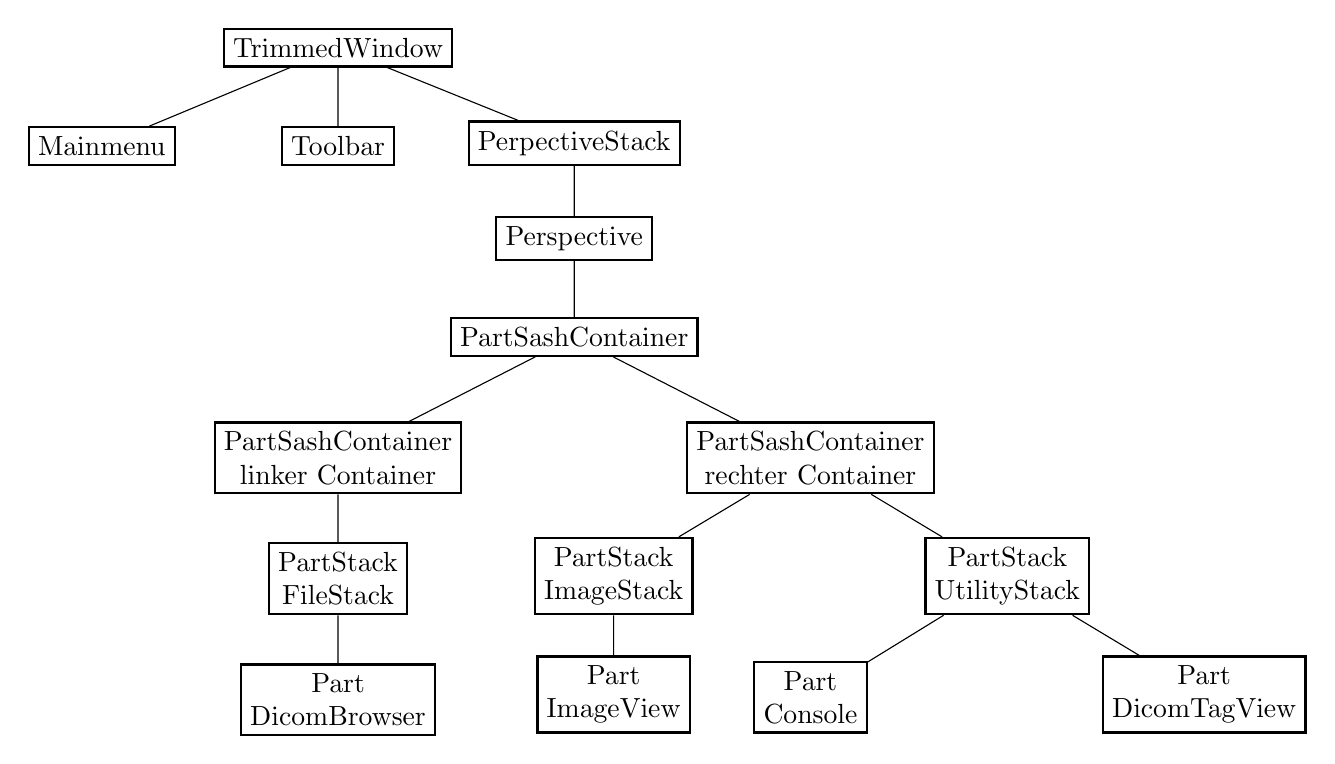
\begin{tikzpicture}[level distance=1.5cm,
  level 1/.style={sibling distance=3cm},
  level 2/.style={sibling distance=5cm},
  level 4/.style={sibling distance = 6cm, level distance = 2cm},
   level 5/.style={sibling distance=5cm},]
  \node {TrimmedWindow}
  child { node{Mainmenu}}
    child { node{Toolbar}}
    child {node {PerpectiveStack}
      child {node{Perspective}
      	child{node{PartSashContainer}
      	  child{node{PartSashContainer \\ linker Container}
      	    child{node{PartStack \\ FileStack}
      	      child{node{Part \\ DicomBrowser}}
      	    }
      	  }
      	  child{node{PartSashContainer \\ rechter Container}
      	    child{node{PartStack \\ ImageStack}
      	      child{node{Part \\ ImageView}}
      	    }
      	    child{node{PartStack \\ UtilityStack}
      	      child{node{Part \\ Console}}
      	      child{node{Part \\ DicomTagView}}
      	    }
      	  }
      	}
      }
    };
\end{tikzpicture}
\end{figure}

\section{Modulare Werkzeuge}
Neben der Applikationsstruktur und deren Implementierung liefern die Werkzeuge weitere grundlegende Funktionen der Anwendung. Damit die Werkzeuge wie die Struktur einen modularen Charakter erhalten, müssen auch diese erweiterbar sein. Ein zusätzliches Problem ist, dass während der Laufzeit nicht bekannt ist, welche Werkzeugobjekte erzeugt werden müssen. Wählt der Anwender aus der Werkzeugleiste ein Tool aus, wird das entsprechende Objekt zum Menüpunkt erzeugt. Ein Klick auf das Translationswerkzeug erzeugt zum Beispiel ein Objekt der Klasse \textit{MoveTool}. Das bedeutet, die Objekterzeugung findet erst nach der Auswahl durch den Benutzer zur Laufzeit statt. Da die Wahl nicht vorbestimmt ist, müssen die konkreten Werkzeugobjekte dynamisch erzeugt werden können. Wie in Abschnitt \ref{fabrikmethod} beschrieben, kann die Fabrik Methode für Anwendungsfälle dieser Art der Objekterzeugung eingesetzt werden. Bei den Klassen selbst wird das Open-Closed-Prinzip beachtet. Die abstrakte Klasse \textit{ATool} gibt ein Grundwerkzeug vor und bietet eine Schnittstelle zur Erweiterung. \textit{AToolFactory} gibt die Vorgehensweise zur Werkzeugerzeugung vor. Abgeleitete Fabriken klassifizieren die Werkzeugkategorien. Durch die Fabrik entsteht eine dynamische Objekterzeugung und die abstrakte Toolklasse liefert die nötige Schnittstelle für eine Erweiterung der Werkzeuge.

%Ein neuer Eintrag in das Hauptmenü und die Werkzeugleiste ist mit Hilfe der Eclipse RCP-Bordmittel schnell erstellt. Dieser %ist allerdings auch unabhängig der bisherigen Menüpunkte. So ist zum Beispiel der Eintrag \textit{Datei öffnen} nicht %abhängig vom Menüpunkt \textit{Einstellungen}. Wird ein Eintrag ausgewählt, wird dieser ausgeführt und das Programm wartet %auf die nächste Eingabe des Benutzers. Schwierigkeiten gibt es bei den Werkzeugen zur Bildmanipulation. Es kann immer nur %ein Werkzeug aktiv ausgewählt sein. Zur Übersetzungszeit ist unklar, welche Werkzeuge wann erzeugt werden müssen. Daraus %folgt, dass die verschiedenen Objekttypen der Werkzeuge erst zur Laufzeit erzeugt werden können, abhängig welches Werkzeug %vom Benutzer ausgewählt wird. Wie in Abschnitt \ref{fabrikmethod} beschrieben, kann die Fabrik Methode für Anwendungsfälle %dieser Art der Objekterzeugung eingesetzt werden. Bei den Klassen wird das Open-Closed-Prinzip beachtet. Die abstrakte %Klasse \textit{ATool} gibt ein Grundwerkzeug vor und bietet eine Schnittstelle zur Erweiterung. \textit{AToolFactory} gibt %die Vorgehensweise zur Werkzeugerzeugung vor. Abgeleitete Fabriken klassifizieren die Werkzeugkategorien.

\begin{figure}[htbp]
  \vspace{0.5cm}
  \centering
  \fbox{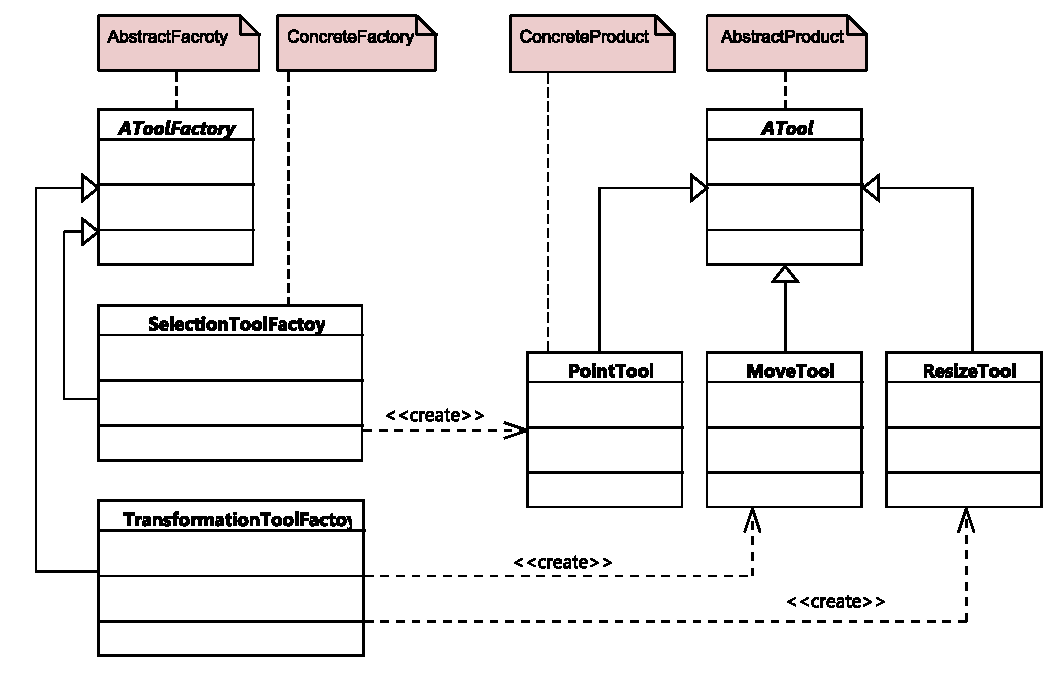
\includegraphics[angle=0,width=12cm]{./img/toolfactory.pdf}}
  \caption{Die Fabrik Methode zur Werkzeugerzeugung}
  %\floatfoot{https://wiki.eclipse.org/Eclipse4}
  \label{toolfactory}
  \vspace{0.5cm}
\end{figure}

Abbildung \ref{toolfactory} zeigt die Umsetzung dieses Erzeugungsmusters. Die Grundversion von jMediKit enthält die zwei konkreten Fabriken \textit{TransformationToolFactory} und \textit{SelectionToolFactory}. Erstere beinhaltet Werkzeuge zur Bildtransformation wie die Skalierung (\textit{ResizeTool}) und letztere enthält ein Werkzeug zur Auswahl von Punkten im Bild(\textit{PointTool}). Sollen weitere Werkzeuge entwickelt werden, können diese von der abstrakten Klasse \textit{ATool} abgeleitet werden und diese erweitern.

\section{Die Plug-in Architektur}

Die Entwicklung von Erweiterungen durch den Anwender spielt neben der Modularität eine weitere Rolle in dieser Abschlussarbeit. Die Entwicklung von zusätzlichen Funktionen und Bedienelemente mittels des Application Models sind erst nach einem erneuten Build-Prozess von jMediKit verfügbar, während Plug-ins auch nach einer Kompilierung des Systems integriert werden können. Es soll den Anwendern eine Möglichkeit geboten werden, eigenständig Erweiterungen zu entwickeln. Der Wirkungsbereich dieser Plug-ins beschränkt sich auf die Manipulation der Bilddaten. Dadurch ist kein explizites Wissen über die Eclipse-Plattform nötig.\\
Die Grundlage der Plug-in Architektur bildet das in Kapitel \ref{swa} vorgestellte Plug-in-Muster. Die Erweiterungen arbeiten im Speziellen mit den Bilddaten. Durch die dreidimensionale Datenstruktur ist es möglich, dass Plug-ins neben der x- und y-Ebene auch in die z-Richtung arbeiten. Dadurch ist eine Anpassung des Architekturmusters notwendig, in der Plug-ins als Typen spezifiziert werden. Als Ergebnis wird eine Kombination aus Plug-in, Schablonenmethode und Singleton eingesetzt. Das UML-Diagramm in Abbildung \ref{aplugin} zeigt die Architektur und Zusammenarbeit der drei Muster.

%Es ergeben sich verschiedene Probleme bei der Umsetzung Schablone, Singleton, 

\begin{figure}[htbp]
  \vspace{0.5cm}
  \centering
  \fbox{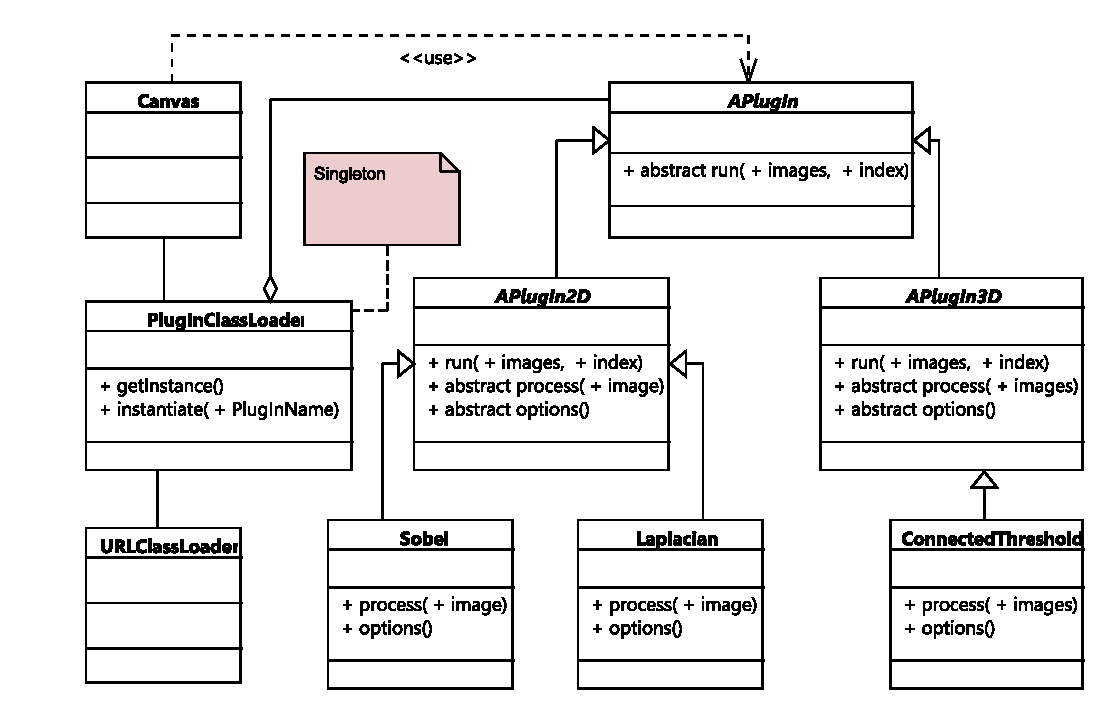
\includegraphics[angle=0,width=12cm]{./img/APlugin.pdf}}
  \caption{Architektur der Plug-in-Struktur}
  %\floatfoot{https://wiki.eclipse.org/Eclipse4}
  \label{aplugin}
  \vspace{0.5cm}
\end{figure}

\subsection{Plug-in als Grundstruktur}
Die Manager-Klasse des Architekturmusters ist \textit{PlugInClassLoader}. Diese Klasse dient sowohl zum Laden der Plug-ins, als auch zum Instantiieren der Plug-in-Objekte. Aufgrund des eingeschränkten Wirkungsbereichs der Plug-ins ist die Zeichenfläche der Anwendung(\textit{Canvas}) das einzige Modul, das über den Manager Plug-in-Objekte erzeugen kann.\\
Ein Unterschied zur UML-Darstellung in Abbildung \ref{pluginpattern} des vorherigen Kapitels besteht darin, dass keine Schnittstelle zur Implementierung, sondern eine abstrakte Klasse \textit{APlugIn} zur Ableitung zur Verfügung gestellt wird. Das bringt den Vorteil, gemeinsame Methoden zu definieren die in allen Plug-ins enthalten sind.
 %jMediKit
%Aufgrund des eingeschränkten Wirkungsbereich der Plug-ins ist die Zeichenfläche der Anwendung das einzige Modul von %jMediKit, das diese Art der Erweiterungen aufrufen ausführen kann. Dadurch besitzt die Manager-Klasse %\textit{PlugInClassLoader} nur eine singuläre Beziehung zur Klasse der Zeichenfläche.

\subsection{Erweiterung mit der Schablonenmethode}
Nach den Anforderungen in Kapitel \ref{anforderungen} ist es nötig, Plug-in-Schnittstellen sowohl für die Entwicklung von zwei- als auch dreidimensionalen Bilddaten anzubieten. Um dies zu erfüllen, stehen dem Benutzer die beiden abstrakten Klassen \textit{APlugIn2D} und \textit{APlugIn3D} zur Verfügung. Beide Varianten repräsentieren die Schablonenmethode. Das Template wird von der Methode \textit{run()} repräsentiert. Der generische Teil des Algorithmus ist \textit{process()}. Die Schablone ist notwendig, da abhängig von 2D und 3D andere Bilddaten an den Benutzer zum Bearbeiten übergeben werden müssen. Nach dem Aufruf von \textit{process()} wird zusätzlich die Rückgabe des Benutzers von der Templatemethode \textit{run()} validiert. Die Schablone ermöglicht dadurch eine Vorverarbeitung und Nachbearbeitung der Bilddaten.
 
\subsection{Singleton als Plug-in Manager}
Der Manager \textit{PlugInClassLoader} ist als Singleton realisiert. Dadurch wird das Problem umgangen, dass mehrere Manager die gleichen Plug-ins laden. Passiert dies, sind gleiche Klassen zueinander inkompatibel und es kann nicht sichergestellt werden, welche Klasse von welchem Manager zur Verfügung gestellt wird.\\
Damit neue Klassen zum Programmstart eingebunden werden können, wird der Java System Classloader über den Manager um einen URL-Classloader erweitert. So werden zu den bisherigen Klassen der Java Virtual Machine alle Plug-in-Klassen hinzugefügt.

\subsection{Plug-ins mit dynamischer Parameterübergabe} \label{genericdialog}

Einen weiteren wichtigen Aspekt der Architektur zur Plug-in-Entwicklung stellt ein generischer Dialog dar. Der Anwender kann dieses Bedienfeld in sein Plug-in einbinden und so eine dynamische Parameterübergabe anstoßen.\\
Das Grundlegende Fenster liefert die Klasse \textit{TitleAreaDialog} aus dem externen SWT- und JFace-Paket. jMediKit erweitert diese Klasse zu einem \textit{PlugInDialog}. Sie enthält eine Liste mit den Schnittstellen \textit{IPlugInDialogItem}. Dieses  Interface liefert die Grundfunktionen der Parametertypen wie zum Beispiel \textit{IntegerItem} und \textit{StringItem}. Der Plug-in-Dialog kann beliebig viele Elemente enthalten.\\
Wird ein Plug-in vom Anwender entwickelt, kann der \textit{PlugInDialog} nicht direkt verwendet werden, da externe Bibliotheken wie SWT und JFace nicht vom Benutzer eingebunden werden und somit die Klassen und Funktionen aufgrund der Abhängigkeiten von \textit{PlugInDialog} und \textit{TitleAreaDialog} nicht aufgelöst werden.
Um dieses Problem zu beheben, wird die weitere Generalisierung \textit{GenericPlugInDialog} eingeführt. Dieser Dialog kann in konkreten Plug-ins instantiiert, angepasst und bearbeitet werden.

\begin{figure}[htbp]
  \vspace{0.5cm}
  \centering
  \fbox{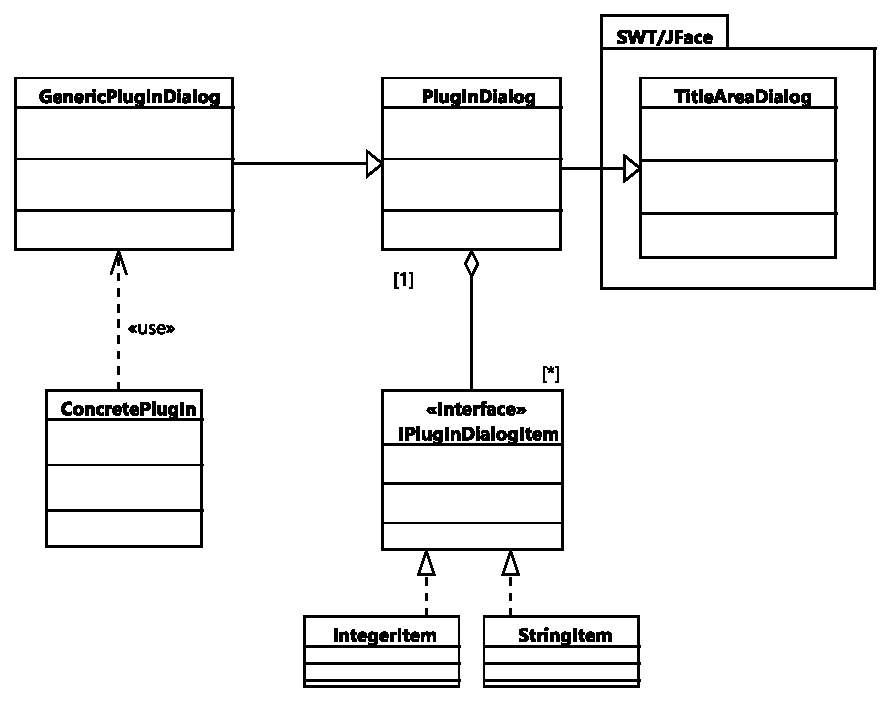
\includegraphics[angle=0,width=9cm]{./img/plugindialog.pdf}}
  \caption{Architektur des generischen Dialogs zur dynamischen Parameterbestimmung}
  %\floatfoot{https://wiki.eclipse.org/Eclipse4}
  \label{plugindialog}
  \vspace{0.5cm}
\end{figure}

\section{Externe Bibliotheken}

Fremde Bibliotheken werden aus verschiedenen Gründen benötigt. Zum einen für das Lesen von DICOM-Objekten und zum anderen bieten Bildverarbeitungsbibliotheken eine gute Grundlage an Funktionen. Zur Verarbeitung von DICOM-Dateien verwendet jMediKit die freie Bibliothek \glqq dcm4che\grqq. Für die Bildverarbeitung wird \glqq Simple ITK\grqq\ eingesetzt.

\subsection{dcm4che}
Im Kapitel \glqq \nameref{grundlagen}\grqq\ wurden die Grundlagen medizinischer Datenformate gezeigt und die Komplexität der Datenstrukturen deutlich gemacht. Eine standardgerechte Implementierung ist daher im Rahmen der Arbeit nicht zufriedenstellend umzusetzen. Dadurch wird zur Verarbeitung medizinischer Daten(vor allem Patienten- und Bilddaten) auf externe Bibliotheken zurückgegriffen. Für eine Implementierung in Java standen als Werkzeuge  \textit{Pixelmed}\footnote{http://www.pixelmed.com/} und \textit{dcm4che2}\footnote{http://www.dcm4che.org/} zur Auswahl. Beide stellen mit einer DICOM-Objekt-Verarbeitung und Netzwerkkommunikation ähnliche Dienste bereit.\\
dcm4che.org bietet allerdings eine Software namens \textit{dcm4chee} um ein PACS zu betreiben. Diese wird im Labor für medizische Bildverarbeitung eingesetzt. Das ermöglicht eine leichtere Integration für spätere Erweiterungen von jMediKit in die bestehende Umgebung des Labors.\\
\textit{dcm4che2} steht unter der GNU General Public License. Dies ermöglicht die freie Verwendung der Software. JMediKit setzt die Version 2.028 ein.

\subsubsection{Java Advanced Imaging Image I/O Tools}
Um alle Bildformate (abhängig von der Transfersyntax der DICOM-Objekte werden Bilddaten komprimiert als JPEG oder JPEG200 gespeichert) lesen zu können, verwendet dmc4che2 die Bildverarbeitungsbibliothek \textit{Java Advanced Imaging Image I/O Tools}. Diese ist \textit{nicht} in dcm4che2 integriert und muss vom Anwender selbst auf dem System installiert werden. Die benötigten Dateien und Pakete können unter \textit{http://download.java.net/media/jai-imageio/builds/release/1.1/ - Stand 31.01.2014} bezogen werden.

\subsection{Simple ITK}
Das \textit{Insight Segmentation and Registration Toolkit(ITK)}\footnote{http://www.itk.org/} ist eine umfangreiche Sammlung an Algorithmen zur Segmentierung und Registrierung. Das ITK ist plattformübergreifend einsetzbar und wurde in C++ implementiert. Zwar sind Java- oder Python-Wrapper\footnote{Wrapper machen es möglich, Bibliotheken fremder Sprachen in aktuellen Sprachen einzubinden und zu benutzen. So wäre es möglich, das ITK, welches in C++ implementiert ist, über Wrapper in Java nutzen zu können.} verfügbar, für die aktuelle Version 4 war es zum Zeitpunkt der Erstellung dieser Arbeit allerdings nicht möglich, zuverlässig einen ITK-Build für eine Verwendung in Java zu erstellen.\\
Das \textit{Simple ITK}\footnote{http://www.simpleitk.org/} bietet eine kompakte Implementierung des ITK. Insgesamt sind 75\% der Klassen aus dem ITK integriert\cite{sitk:filter}. Für einen Einsatz in einer Java Umgebung, kann das Projekt als Java-Bibliothek bezogen werden. Simple ITK steht unter der Apache 2.0 Lizenz und erlaubt eine uneingeschränkte Nutzung.

\subsection{Der Adapter zur Auflösung von Abhängigkeiten} \label{adapter_dependencies}

Eine Nutzung von externen Bibliotheken bedeutet gleichzeitig, dass Abhängigkeiten zwischen dem zu entwickelnden Programm und den fremden Paketen geschaffen werden. Werden bibliotheksspezifische Objekte im Quelltext erzeugt ist man abhängig von einer kontinuierlichen Weiterentwicklung der eingebundenen Projekte. Bei einem Wechsel der Bibliotheken müssen alle referenzierten Objekte angepasst werden und der Code ist nur mit einem erheblichen Mehraufwand wartbar.\\
Mit Hilfe des Adapters werden bei jMediKit die Abhängigkeiten aufgelöst. In Abbildung \ref{dicomo} wird das Klassendiagramm dargestellt. Wie das Plug-in Muster, wird auch der Adapter mit Anpassungen eingesetzt. Unter jMediKit wird ein DICOM-Objekt aus zwei unterschiedlichen Teilen repräsentiert. Ein Teil beinhaltet den reinen Datenteil (\textit{IDicomData}). Das bedeutet, alle verfügbaren Tags des DICOM-Objekts sind enthalten. Der zweite Teil besteht aus den reinen Pixeldaten (IDicomImageData). Diese beiden Schnittstellen bilden den Adapter für die externe Bibliothek \textit{dcm4che2}. Durch die Trennung von Daten und Bilddaten bleibt die Flexibilität bei der Bibliothekswahl erhalten. So kann zum Beispiel Simple ITK nur für das Einlesen der Bilddaten verwendet werden, denn es werden keine Methoden zum Auslesen der Tags geboten. Dadurch wäre eine zweite Bibliothek für den Datenteil notwendig. In der Implementierung des Adapters wird in beiden Teilen \textit{dcm4ch2} eingesetzt, da diese Bibliothek sowohl Daten als auch Bilddaten verarbeiten kann. Die beiden Klassen \textit{DicomImageData} und \textit{DicomData} implementieren die Schnittstellten \textit{IDicomImageData} und \textit{IDicomData}. Keine anderen Klassen greifen auf Objekte und Methoden aus den Bibliotheken zu.\\
Um beide Aspekte zu vereinen, stellen die Schnittstellen \textit{IDicomData} und \textit{IDicomImageData} die neuen zu adaptierenden Funktionen dar, die von \textit{ADicomObject} adaptiert werden. Der konkrete Adapter ist \textit{DicomObject}. Um die Abhängigkeiten aufzulösen und die Flexibilität in der Bibliothekswahl zu wahren, wird dieser geschachtelte Adapter eingesetzt.

\begin{figure}[htbp]
  \vspace{0.5cm}
  \centering
  \fbox{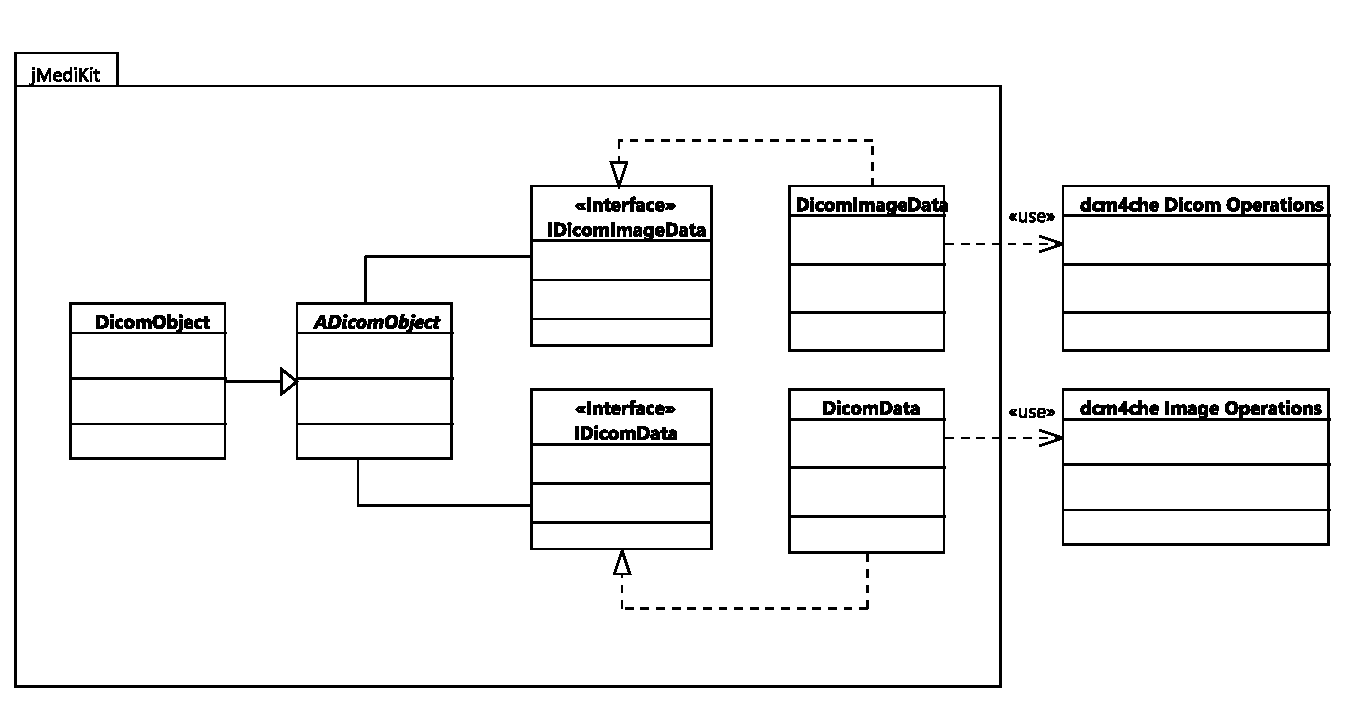
\includegraphics[angle=0,width=12cm]{./img/Dicomo.pdf}}
  \caption{Das Adapter-Muster unter jMediKit}
  %\floatfoot{https://wiki.eclipse.org/Eclipse4}
  \label{dicomo}
  \vspace{0.5cm}
\end{figure}

Zusätzlich wird die Schnittstelle zur Bibliothek vereinfacht, indem nur Funktionen zur Verfügung gestellt werden, die tatsächlich eingesetzt werden. Werden zusätzliche Funktionen benötigt, kann das Interface der Adapter erweitert werden.\\
Soll zukünftig eine Bibliothek getauscht werden, muss nur das Interface neu implementiert werden und die Anwendung kann wie gewohnt eingesetzt werden.

\section{Die Architektur der Bilddaten}

Die Bilddaten sind ein Teil des Adapters \textit{ADicomObject} des Java Medical Imaging Toolkits. Diese werden mit Hilfe der abstrakten Klasse \textit{AImage} dargestellt und enthalten viele zusätzliche Informationen wie Bilddimension, Fensterungsdaten oder die Position des Patienten im Raum. \textit{AImage} repräsentiert die Grundlage einer Bildrepräsentation von jMediKit. Wie in Kapitel \ref{grundlagen} erläutert, besitzen medizinische Bilder unterschiedliche Grauwert-Tiefen oder Farbdarstellungen. Um die unterschiedlichen Bildtypen abzubilden, stehen die konkreten Klassen \textit{UnsignedByteImage} $\rightarrow$ 8-Bit, \textit{ShortImage} $\rightarrow$ 16-Bit, \textit{UnsignedShortImage} $\rightarrow$ 16-Bit und \textit{IntegerImage} $\rightarrow$ 32-Bit Farbbild zur Verfügung. Ein \textit{ADicomObject} beinhaltet alle Bilddaten der entsprechenden Serie des DICOM-Objekts.\\
Um mit \textit{AImage} zu arbeiten gibt es zwei Möglichkeiten: Die Erste ist das Auslesen über das \textit{ADicomObject}. Hierzu muss ein DICOM-Objekt aus einer Datei eingelesen werden. Im Bereich der Plug-in-Entwicklung ist es sinnvoll leere Bilder zu erzeugen und während der Anwendung des Plug-ins mit neuen Werten zu Füllen. Hierbei hilft die Klasse \textit{SimpleImageFactory}.

\begin{figure}[htbp]
  \vspace{0.5cm}
  \centering
  \fbox{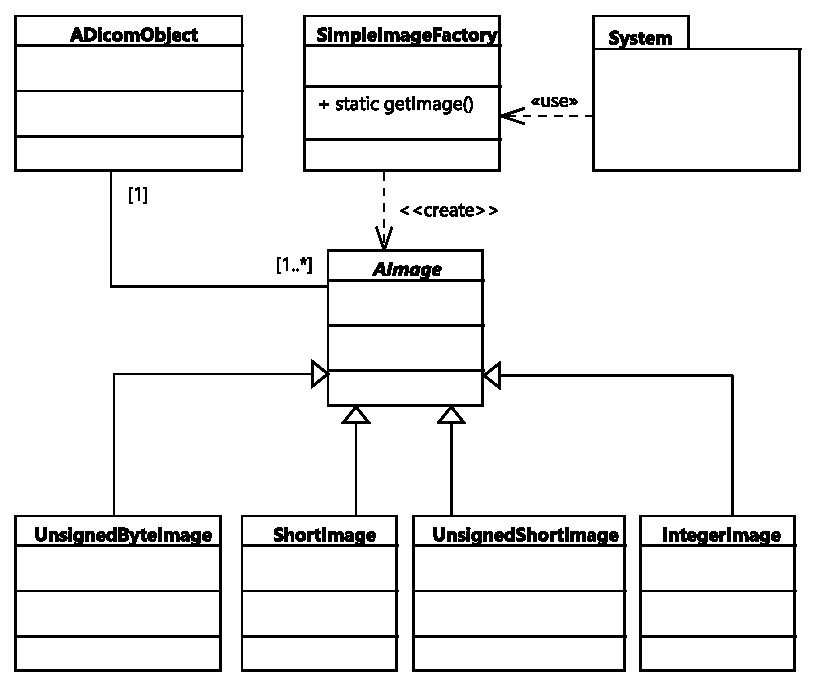
\includegraphics[angle=0,width=12cm]{./img/imagemodel.pdf}}
  \caption{Diagramm zur Klassenstruktur der Bilddaten}
  %\floatfoot{https://wiki.eclipse.org/Eclipse4}
  \label{imagemodel}
  \vspace{0.5cm}
\end{figure}

\subsection{Die einfache Fabrik}

Die einfache Fabrik ähnelt der Fabrikmethode, allerdings wird dieses Verfahren der Objekterzeugung nicht den Entwurfsmustern zugeordnet.\\
Beim Entwickeln von Plug-ins können Anwender vor dem Problem stehen, nicht zu wissen, welche Grauwert-Tiefe das aktuell geladene Objekt besitzt. Nur ein mühsames Auslesen über die DICOM-Tags und einer Schleife zur Typ-Ermittlung würde Abhilfe schaffen. Da die Bilder bereits in den Speicher geladen wurden, ist dem System implizit der Bildtyp bekannt, jedoch nicht explizit dem Anwender. Durch die Übergabe eines bereits geladenen Bildes, kann ein neues Bild vom richtigen Typ, ohne explizites Wissen des Nutzers, erzeugt werden.

% Der statischen Methode \textit{getImage()} von \textit{SimpleImageFactory} kann der Bildtyp des DICOM-Objekts übergeben % % werden, worauf ein typgerechtes Bildobjekt erzeugt und zurückgegeben wird.

\subsection{Struktur der Bilder im ImageViewPart} \label{ivp_architecture}

Da die Struktur der Bilddaten dargestellt wurde, kann nun die Vorgehensweise zur Anzeige dieser vorgestellt werden.\\

\begin{figure}[htbp]
  \vspace{0.5cm}
  \centering
  \fbox{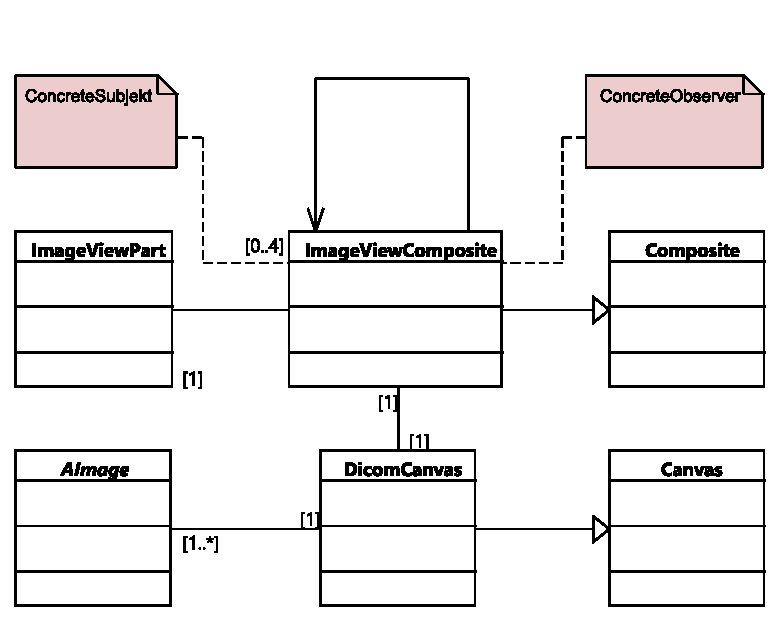
\includegraphics[angle=0,width=12cm]{./img/imageview.pdf}}
  \caption{Organisation der Klassen zur Anzeige der DICOM-Bilddaten}
  %\floatfoot{https://wiki.eclipse.org/Eclipse4}
  \label{imageview}
  \vspace{0.5cm}
\end{figure}

Auf der Benutzeroberfläche findet dieser Vorgang im ImageView Part statt (Abschnitt \ref{hierarchyextending}). Wie in Abbildung \ref{imageview} zu sehen, bildet \textit{ImageViewPart} die Grundlage und dient als Elternelement eines \textit{ImageViewComposites}, von denen mehrere zum gleichen Zeitpunkt angezeigt werden können. \textit{ImageViewComposites} erben von der SWT-Klasse \textit{Composite} und enthalten weitere Bedienelemente für den Benutzer. Hierzu zählt die Scrollleiste am rechten Rand wie in Abbildung \ref{iv:1} zu sehen ist. Mit diesem Scrollbalken wird die Schicht aus den dreidimensionalen Bilddaten gewählt, die vom \textit{DicomCanvas} angezeigt werden soll. Die Superklasse von \textit{DicomCanvas} gehört ebenfalls zum Repertoire des SWT und ist das zentrale Element zur Bildanzeige. \textit{DicomCanvas} enthält sämtliche Bilder des DICOM-Objekts.

\begin{figure*}[htb]
%\subfigure[Keypoints]{\includegraphics[width=0.49\textwidth]{./img/basmati_keypoints.png}}\hfill
\centering
\fbox{
\subfigure[Darstellung eines ImageViewComposite]{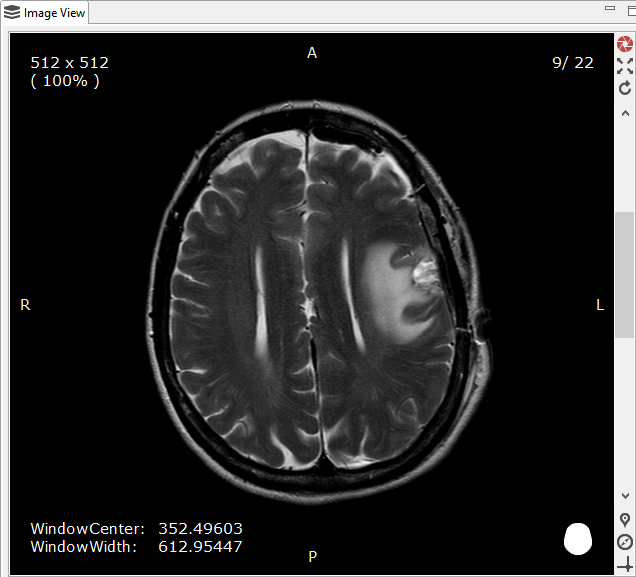
\includegraphics[width=0.5\textwidth]{./img/ivcomposite.png} \label{iv:1}}
\subfigure[Vier ImageViewComposites im ImageViewPart]{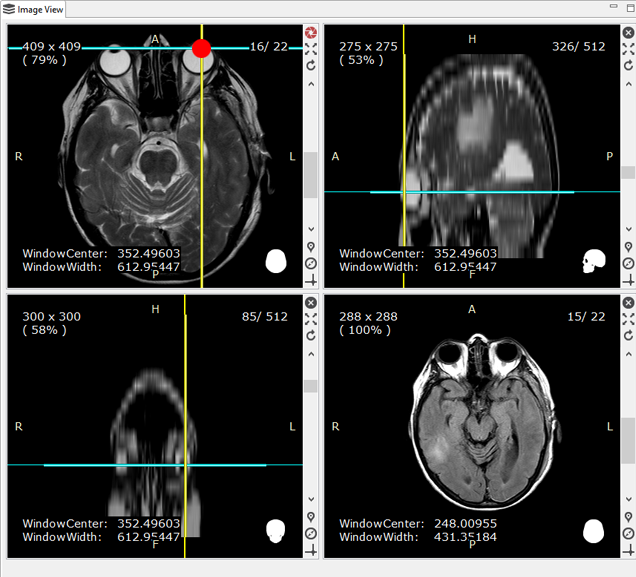
\includegraphics[width=0.5\textwidth]{./img/ivcomposite4.png} \label{iv:4}}
}
\caption{Benutzeroberfläche der ImageViewComposites}
\label{ivcomposite}
\end{figure*}

Abbildung \ref{iv:4} zeigt vier \textit{ImageViewComposites}, wobei alle außer Composite unten rechts die gleichen DICOM-Objekte anzeigen.
Angenommen ein Benutzer führt einen Klick mit der rechten Maustaste auf den in rot markierten Punkt aus, müssen alle \textit{ImageViewComposites} den gleichen Punkt im dreidimensionalen Raum referenzieren. Dieser wird durch den Schnittpunkt der Linien angezeigt. Eine genaue Beschreibung dazu befindet sich in Kapitel \ref{implementation}.\\
Damit dieses Verhalten von Seiten der Architektur unterstützt wird, muss sichergestellt werden, dass die \textit{ImageViewComposites} untereinander kommunizieren können, dass eine Änderung stattgefunden hat.\\
Aus dem Kapitel \ref{swa} löst das Observer-Muster diese Anforderungen. Der Zyklus in Abbildung \ref{imageview} repräsentiert das Muster und zeigt die Funktionsweise. Jede ImageViewComposite ist gleichzeitig \textit{ConcreteSubject} als auch \textit{ConcreteObserver}. Das bedeutet, bei jeder Registrierung eines neuen DICOM-Objekts wird geprüft, ob dieses schon im \textit{ImageViewPart} vorhanden ist. Ist dies der Fall, wird es als neuer Observer an bisherigen Subjects angemeldet.\\
Bei diesem Einsatz besteht die Gefahr einer Endlosschleife, wenn der Zyklus nicht beachtet wird. Die Schleife tritt ein, wenn ein Subject die Observer benachrichtigt, die Observer ändern den Status und benachrichtigen darauf wiederum ihre Beobachter und so weiter. Bei der Implementierung von jMediKit wird eine Änderung angenommen und das \textit{DicomCanvas} neu gezeichnet und löst keine Rückmeldung einer Änderung aus. \\
Auf dieser Architekturgrundlage findet die im folgenden Kapitel erläuterte Implementierung statt.